% 专题四：极值与最值
\section{专题四：极值与最值}

\begin{learnobjective}
\begin{itemize}
  \item 会配方求二次函数的最值，并说明最值的位置；
  \item 会用单调性判断区间上的最值；
  \item 会用导数求一般函数的极值；
  \item 会用线性规划求带约束的最值。
\end{itemize}
\end{learnobjective}

\begin{preview}
\subsection{导语：同一个问题，五种看法}
最值问题在小学就遇到过（面积最大、用料最省），
中学用二次函数求最值，高中用导数求一般函数的极值，再往后用线性规划处理带约束的最值。
同一个“最大 / 最小”问题，工具会不断升级。
本专题把三个“种子问题”用五种视角各做一遍。

\subsection{种子问题}
先自己做，再看后面的五种视角。
\begin{enumerate}
  \item 求 $f(x)=x^2-2x-3$ 的最小值。
  \item 求 $f(x)=x^2-2x-3$ 在 $[0,4]$ 上的最大值与最小值。
  \item 用长为 $L$ 的铁丝围成一个矩形，求面积的最大值。
\end{enumerate}
\end{preview}

\begin{explore}
\subsection{视角一：来源——最值问题从哪来}

\key{要点}
\begin{itemize}
  \item 实际问题中的优化：面积最大、用料最省、利润最大、成本最低。
  \item 数学上，这些问题都可以写成“在某个范围内，求某个量的最大值或最小值”。
\end{itemize}

\begin{example}
用长为 $L$ 的铁丝围成一个矩形，求面积的最大值。
\end{example}
\begin{solution}
设矩形一边长为 $x$，则另一边长为 $\dfrac{L}{2}-x$（$0<x<\dfrac{L}{2}$），
面积 $S=x\left(\dfrac{L}{2}-x\right)=-\left(x-\dfrac{L}{4}\right)^2+\dfrac{L^2}{16}$。
故当 $x=\dfrac{L}{4}$（即为正方形）时，面积最大，最大值为 $\dfrac{L^2}{16}$。
\key{（回头看：种子问题 3）}
\end{solution}

\begin{problem}
用长为 $20\ \mathrm{cm}$ 的铁丝围成一个矩形，面积最大是多少？
\end{problem}
\begin{solution}
$S=x(10-x)=-(x-5)^2+25$，当 $x=5$ 时取最大值 $25\ \mathrm{cm^2}$。
\end{solution}

\subsection{视角二：证明——为什么最值在那个位置}

\key{要点}
\begin{itemize}
  \item 二次函数开口向上时，顶点是最小值点（用配方法可证）；开口向下时，顶点是最大值点。
  \item 闭区间上的连续函数必有最大值和最小值；对二次函数，最值只可能在顶点或区间端点处取得。
\end{itemize}

\begin{example}
用配方法证明：$f(x)=x^2-2x-3$ 的最小值为 $-4$。
\end{example}
\begin{solution}
$f(x)=x^2-2x-3=(x-1)^2-4$。因为 $(x-1)^2\geq0$，所以 $f(x)\geq-4$，
当 $x=1$ 时取等号。故最小值为 $-4$。
\key{（回头看：种子问题 1）}
\end{solution}

\begin{problem}
用配方法证明：$f(x)=2x^2-4x+1$ 的最小值为 $-1$。
\end{problem}
\begin{solution}
$f(x)=2(x-1)^2-1\geq-1$，当 $x=1$ 时取等号。
\end{solution}

\subsection{视角三：函数——用单调性看最值}

\key{要点}
\begin{itemize}
  \item 先减后增的函数，在转折点（顶点）处取最小值；
  \item 最大值看区间端点：开口向上时，离对称轴越远的端点值越大。
\end{itemize}

\begin{example}
求 $f(x)=x^2-2x-3$ 在 $[0,4]$ 上的最大值与最小值。
\end{example}
\begin{solution}
对称轴 $x=1\in[0,4]$，最小值为 $f(1)=-4$。
端点值 $f(0)=-3$，$f(4)=5$；$4$ 离对称轴更远，故最大值为 $f(4)=5$。
\key{（回头看：种子问题 2）}
\end{solution}

\begin{problem}
求 $f(x)=-x^2+4x+1$ 的最大值。
\end{problem}
\begin{solution}
$f(x)=-(x-2)^2+5$，开口向下，故当 $x=2$ 时取最大值 $5$。
\end{solution}

\subsection{视角四：极值——求极值的方法}

\key{要点}
\begin{itemize}
  \item \key{配方法 / 顶点公式}：二次函数在 $x=-\dfrac{b}{2a}$ 处取最值。
  \item \key{导数法}：令 $f'(x)=0$ 求驻点，再看 $f'$ 在驻点两侧的符号变化。
  \item \key{判别式法}：形如 $y=\dfrac{ax^2+bx+c}{dx^2+ex+f}$ 的函数，化为关于 $x$ 的二次方程，用 $\Delta\geq0$ 求值域。
\end{itemize}

\begin{example}
用导数求 $f(x)=x^3-3x^2+2$ 的极值。
\end{example}
\begin{solution}
$f'(x)=3x^2-6x=3x(x-2)$。
当 $x<0$ 时 $f'(x)>0$；$0<x<2$ 时 $f'(x)<0$；$x>2$ 时 $f'(x)>0$。
故 $x=0$ 处取极大值 $f(0)=2$，$x=2$ 处取极小值 $f(2)=-2$。
\end{solution}

\begin{problem}
用判别式法求函数 $y=\dfrac{x^2+x+1}{x^2+1}$ 的值域。
\end{problem}
\begin{solution}
由 $y(x^2+1)=x^2+x+1$ 得 $(y-1)x^2-x+(y-1)=0$。
$y=1$ 时方程为 $-x=0$，有解 $x=0$，故 $y=1$ 可取；
$y\neq1$ 时，$\Delta=1-4(y-1)^2\geq0$，解得 $\dfrac12\leq y\leq\dfrac32$。
综上，值域为 $\left[\dfrac12,\dfrac32\right]$。
\end{solution}

\key{（回头看：用导数法求种子问题 1 的最小值，结果应与配方法一致）}

\subsection{视角五：几何——带约束的最值（线性规划）}

\key{要点}
\begin{itemize}
  \item 约束条件（不等式组）给出可行域；目标函数的等值线是一族平行直线。
  \item 线性目标函数在可行域上的最值，在顶点处取得。
\end{itemize}

\begin{figure}[htbp]
  \centering
  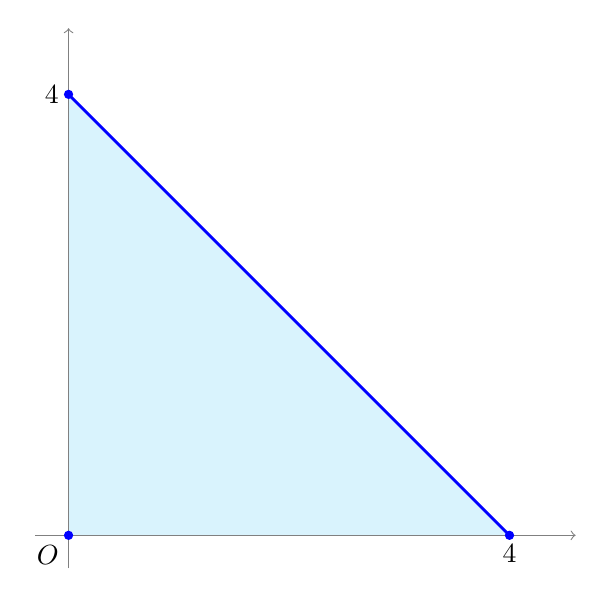
\begin{tikzpicture}[scale=1.4]
    \fill[cyan!15] (0,0) -- (4,0) -- (0,4) -- cycle;
    \draw[->, gray] (-0.3,0) -- (4.6,0);
    \draw[->, gray] (0,-0.3) -- (0,4.6);
    \draw[blue, line width=1pt] (4,0) -- (0,4);
    \fill[blue] (0,0) circle (1.2pt);
    \fill[blue] (4,0) circle (1.2pt);
    \fill[blue] (0,4) circle (1.2pt);
    \node[below] at (4,0) {$4$};
    \node[left] at (0,4) {$4$};
    \node[below left] at (0,0) {$O$};
  \end{tikzpicture}
  \caption{不等式组 $x+y\leq4,\ x\geq0,\ y\geq0$ 表示的可行域}
\end{figure}

\begin{example}
设 $x+y\leq4$，$x\geq0$，$y\geq0$，求 $z=x+y$ 的最大值。
\end{example}
\begin{solution}
可行域是以 $(0,0)$、$(4,0)$、$(0,4)$ 为顶点的三角形。
$z=x+y$ 在三点处的值分别为 $0$、$4$、$4$，故最大值为 $4$。
\end{solution}

\begin{problem}
设 $x+y\leq4$，$x-y\leq0$，$x\geq0$，$y\geq0$，求 $z=2x+y$ 的最大值。
\end{problem}
\begin{solution}
可行域以 $(0,0)$、$(0,4)$、$(2,2)$ 为顶点。
$z=2x+y$ 在三点处的值分别为 $0$、$4$、$6$，故最大值为 $6$（在 $(2,2)$ 处取得）。
\end{solution}

\key{（回头看：种子问题 3 中，若把目标改为线性式 $z=x+2y$，约束 $x+y=\dfrac{L}{2}$ 下的最值在何处取得？）}
\end{explore}

\begin{inclasstest}
\subsection{变式训练}
只改一个条件，重新做一遍。
\begin{enumerate}
  \item 求 $f(x)=x^2-2x+3$ 在 $[-1,2]$ 上的最大值与最小值。
  \item 用导数求 $f(x)=x^3-6x^2+9x$ 的极值。
  \item 设 $x+y\leq4$，$x\geq0$，$y\geq0$，求 $z=x+2y$ 的最大值。
  \item 用长为 $24\ \mathrm{cm}$ 的铁丝围成一个矩形，面积最大是多少？
\end{enumerate}
\end{inclasstest}

\begin{afterclass}
\subsection{知识来源对照表}
\begin{center}
\footnotesize
\setlength{\tabcolsep}{4pt}
\renewcommand{\arraystretch}{1.35}
\begin{tabular}{p{3.4cm}p{4.0cm}p{5.6cm}}
\toprule
结论 / 方法 & 最早从哪来 & 后面从哪个角度看 \\
\midrule
配方求最值 & 视角一（来源） & 视角二（证明）、视角四（极值） \\
顶点公式 & 视角二（证明） & 视角三（函数）、视角四（极值） \\
单调性定最值位置 & 视角三（函数） & 视角四（极值） \\
导数求极值 & 视角四（极值） & 视角三（函数） \\
判别式法 & 视角四（极值） & 视角二（证明） \\
线性规划 & 视角五（几何） & 视角四（约束最值） \\
\bottomrule
\end{tabular}
\end{center}

\key{下一步}：三个专题（不等式、函数与方程、极值与最值）已跑通同一套结构，
后续可继续补充新主题。
\end{afterclass}
